\section{Extended Example: Class Infrastructure for a Multi-player Game}

In this example, we develop some classes that may support a multi-player game, and we apply some visualization concepts in drawing a rudimentary game arena with avatars representing players. Therefore, we begin by defining an \texttt{Avatar} class. The example will continue with visualization of multiple avatars within a single \texttt{axes} object.

\subsection{Defining an \texttt{Avatar} Class}

We show a rudimentary \texttt{Avatar} class definition in Listing \ref{AvatarClassDef0}. Properties typical of a player's digital representation in a role-playing video game are present. The constructor method allows several different invocation syntaxes. Also, we have defined a \texttt{move()} method, which is used to change the \texttt{Avatar} object's position on the battlefield.
% vvv------------------------------------------------------------vvv
\begin{lstlisting}[style=Matlab-editor, label=AvatarClassDef0, caption={An initial class definition file for the \texttt{Avatar} class.}]
classdef Avatar
    %AVATAR objects represent a player in a multi-player role-playing game.
    %   The AVATAR class defines properties typical of avatars in RPGs.
    %
    % By E.P. Blair
    % Baylor University
    
    properties
        Name = 'Unidentified Player';
        Class % {'mage', 'warrior', 'thief', 'jedi', 'sith', 'none'}
        Level = 1; % a numerical rank for a player
        Position = [0 0]; % (x, y) double for
        XP = 0; % a numerical property for accumulating experience points
        HealthPointsMax = 100; % player's maximum health points (HP)
        Vitality = 1 % player's actual vitality (fraction of maximum vitality)
                     % HP = Vitality * HealthPointsMax
        Attack % numerical rating for offensive capabilities
        Defense % numerical rating for densive capabilities
        WeaponList % list of player's a offensive equipment
        ArmorList % list of player's a defensive equipment
        EquipmentList % list of player's equipment items
    end % END: properties
    
    methods
        function obj = Avatar(varargin)
            %Avatar instantiates an AVATAR object
            %   SYNTAX
            %
            %   newAvatar = Avatar creates a default AVATAR object
            %
            %   newAvatar = Avatar(Username) creates a default AVATAR
            %          object and specifies Username as the name.
            %
            %   newAvatar = Avatar(Username, PlayerClass) creates a default
            %           AVATAR object with name Username and class
            %           PlayerClass.
            %
            
            switch nargin
                case 0
                    obj.Class = 'none';
                case 1
                    obj.Name = varargin{1};
                    obj.Class = 'none';
                case 2
                    obj.Name = varargin{1};
                    obj.Class = varargin{2};
            end
        end
        
        function obj = move(obj, dispVect)
            % myPlayer = myPlayer.move( [dX dY] ) displaces the avatar on
            %   the battlefield.
            obj.Position = obj.Position + dispVect;
        end
        
        function disp(obj)
            % disp(someAvatar) is the display function for the AVATAR
            % class.
            disp([obj.Name, ' (Level ', num2str(obj.Level), ' ', ...
                obj.Class, ') is at (', ...
                num2str(obj.Position(1)) , ', ', ...
                num2str(obj.Position(2)), ').']);
        end
        
    end % END: methods
end
\end{lstlisting}
% ^^^------------------------------------------------------------^^^

\subsubsection{Overriding the \texttt{disp()} Function}
We also have defined a \texttt{disp()} function. Each bulit-in MATLAB class has its own particular \texttt{disp} function, which is invoked to display information about an object in question when an unsuppressed MATLAB calculation yields an object of that class. For a user-defined class, if no \texttt{disp()} method is defined, MATLAB displays that object in a manner similar to the display of a \texttt{struct}, giving a listing of all of the fields pertinent to that particular class. Here, we have a customized \texttt{disp()} method that is written to display the player's name, level and class, as well the battlefield position of the player's \texttt{Avatar} object. When a method \texttt{someMethod()} is defined for a class, but \texttt{someMethod()} already exists for other classes, we say that we have \textbf{overridden} the \texttt{someMethod()} method. Here, we have overridden the \texttt{disp} method to define a customized format for the display of information for objects of class \texttt{Avatar}.

As an example, see Listing \ref{AvatarClassDefTestCmdWin01}, where we test the new \texttt{Avatar} class definition in the Command Window. When the \texttt{Avatar} constructor is invoked (and not suppressed), the result is an object of class \texttt{Avatar}, so the \texttt{Avatar} class \texttt{disp()} method is invoked to display information about the resulting \texttt{Avatar} object:
% vvv------------------------------------------------------------vvv
\begin{lstlisting}[style=Matlab-editor, label=AvatarClassDefTestCmdWin01, caption={Command Window input and output to test the \texttt{Avatar} class constructor and overridden \texttt{disp()} method.}]
>> newAvatar = Avatar('Sargon', 'warrior')

newAvatar = 

Sargon (Level 1 warrior) is at (0, 0).
\end{lstlisting}
% ^^^------------------------------------------------------------^^^

\subsubsection{Testing the \texttt{move()} Method}
Next, we test the \texttt{move()} method in the Command Window:
% vvv------------------------------------------------------------vvv
\begin{lstlisting}[style=Matlab-editor, label=AvatarClassDefTestCmdWin02, caption={The \texttt{Avatar} class \texttt{move()} method worked as desired in a Command Window test.}]
>> newAvatar = newAvatar.move([27, -126])

newAvatar = 

Sargon (Level 1 warrior) is at (27, -126).
\end{lstlisting}
% ^^^------------------------------------------------------------^^^

\subsection{Graphical Visualization for the \texttt{Avatar} Class}

This is where writing the \texttt{Avatar} class gets fun and challenging. First, we will add a \texttt{draw()} method which draws a graphical representation of an \texttt{Avatar} object on an axes. This calls for adding a property to the \texttt{Asset} class which stores a handle to the drawing. When the \texttt{draw()} method is invoked, it can then check to see if the \texttt{Avatar} object already has a drawing; if so, we need not draw it again. Then, we will upgrade the \texttt{move()} method so that it not only changes the \texttt{Position} property, but also updates the \texttt{Avatar} object's drawing, as applicable.

% ============================================
% ============================================
\subsection{The \texttt{Avatar} Class \texttt{draw()} Method}
% ============================================
% ============================================
Listing \ref{AvatarClassDef01} shows the new snippets of the \texttt{Avatar} class definition file.
% vvv------------------------------------------------------------vvv
\begin{lstlisting}[style=Matlab-editor, label=AvatarClassDef01, caption={A \texttt{draw()} method was added to the \texttt{Avatar} class.}]
classdef Avatar
    %AVATAR objects represent a player in a multi-player role-playing game.
    %   The AVATAR class defines properties typical of avatars in RPGs.
    %
    % By E.P. Blair
    % Baylor University
    
    properties
        
        <-- snip -->        

        % Graphics-related properties
        Drawing % A struct of handles to the drawing components
        
    end % END: properties
    
    methods

        <-- snip -->        
                
        function obj = draw(obj, varargin)
            
            % Default values 
            TargetAxes = [];
            % Override default values: parse varargin for property-value
            %   pairs
            
            args = varargin;
            while length(args) >= 2
                prop = args{1};
                val = args{2};
                args = args(3:end);
                
                switch prop
                    case 'Axes'
                        TargetAxes = val;
                    otherwise
                        error(['''', prop, ''' is an invalid ', ...
                            'property specifier.'])
                end % END switch prop
            end % END while length(args) >= 2 
            
            if isempty(obj.Drawing)
                
                % DRAW THE SQUARE (MAIN BODY)
                % Calculate relative points of corners
                x_rel = [-5 -5 5 5];
                y_rel = [-5 5 5 -5];
                % Calculate absolute points of corners
                x = obj.Position(1) + x_rel;
                y = obj.Position(2) + y_rel;
                % visualization
                Drawing.Body = patch(x, y, [1 1 1], ...
                    'EdgeColor', [0 0 0], 'LineWidth', 2);

                NameText = text(obj.Position(1), obj.Position(2), ...
                    obj.Name, 'FontName', 'Times', 'FontSize', 18, ...
                    'HorizontalAlignment', 'center', ...
                    'VerticalAlignment', 'bottom');
                
                % PLAYER INFO STRING
                % 'LVL. X C' (X = Level, C = Class)
                PlayerInfoStr = ['LVL. ', num2str(obj.Level), ' ', ...
                    upper(obj.Class(1:3))];
                xPInfoStr = obj.Position(1);
                yPInfoStr = obj.Position(2) + 4;
                PlayerInfoText = text(xPInfoStr, yPInfoStr, PlayerInfoStr, ...
                    'FontName', 'Times', 'FontSize', 14, ...
                    'HorizontalAlignment', 'center', ...
                    'VerticalAlignment', 'middle');
                
                
                % HEALTH BAR
                % Full health will span [-4, 4] (relative)
                % No health is a point at -4 (relative
                % Color will transition from [0 0.5 0] (green, full)
                % to [1 0 0] (red, empty)
                cHealthLine = [ 1-obj.Vitality, 0.75*obj.Vitality, 0];
                xHealthLine = obj.Position(1) + [-4, -4+8*obj.Vitality];
                yHealthLine = obj.Position(2) - [2 2];
                HealthLine = line( xHealthLine, yHealthLine, ...
                    'Color', cHealthLine, ...
                    'LineWidth', 5);

                % HEALTH STATUS STRING (HealthStr)
                % 'HP: XX/MAX'
                HealthStr = ['HP: ', ...
                    num2str(round(obj.Vitality*obj.HealthPointsMax)), ...
                    '/', num2str(obj.HealthPointsMax)];
                xHealthStr = obj.Position(1) + 4;
                yHealthStr = obj.Position(2) - 3.5;
                HealthText = text(xHealthStr, yHealthStr, HealthStr, ...
                    'FontName', 'Times', 'FontSize', 14, ...
                    'HorizontalAlignment', 'right', ...
                    'VerticalAlignment', 'middle');

                % Populate the Drawing struct
                Drawing.PlayerInfoText = PlayerInfoText;
                Drawing.HealthText = HealthText;
                Drawing.Health = HealthLine;
                
                % store Drawing in obj.Drawing
                obj.Drawing = Drawing;
                
            end
        end
        
    end % END: methods
end
\end{lstlisting}
% ^^^------------------------------------------------------------^^^
The \texttt{draw()} method provides some nice features here:
\begin{itemize}
\item \texttt{draw()} supports optional property-value pairs using \texttt{varargin}. A block is reserved for default values (lines 22-23), which then can be optionally overridden by using the property-value pairs (lines 28-41).
\item Line 43 is used to evaluate whether drawing is necessary. Drawing only commences if the \texttt{obj.Drawing} object is empty, which is the case for any newly-created \texttt{Avatar} object (see the newly-added \texttt{Drawing} property on line 13).
\item Drawing begins with a square patch of side length 10, centered at the \texttt{Avatar} object's position (lines 45-54).
\item \texttt{draw()} writes the character's name in the center of the square patch. See lines 56-59.
\item \texttt{draw()} provides a player information string, with character level and the first three letters of the character class. See lines 61-70.
\item A health bar is shown below the character name. Its length decreases as the character's vitality decreases from full health (\texttt{Vitality = 1}) to no health (\texttt{Vitality = 0}). Additionally, the health bar will turn red as \texttt{Vitality} approaches 0. See lines 73-83.
\item A health string is shown at the bottom, including the current number of health points and the maximum number of health points for the player (lines 85-96).
\end{itemize}

Thus, the result of the testbed function \texttt{testbedAvatar.m} (Listing \ref{AvatarDrawTestbed}) is the MATLAB \texttt{figure} shown in Fig.\ \ref{fig:AvatarDrawing}. At this point, the \texttt{draw()} method seems to work as well as designed. Next steps include:
\begin{itemize}
\item Upgrading the \texttt{move()} method to update the graphics objects stored within the \texttt{Drawing} property.
\item Adding functions such an \texttt{updateStatus()} method, which and update the data represented in the drawing. This method also could be called by other methods, such as \texttt{injure()} and \texttt{heal()}, which adjust the player's \texttt{Vitality} property, along with updating the drawing data.
\end{itemize}
% vvv------------------------------------------------------------vvv
\begin{lstlisting}[style=Matlab-editor, label=AvatarDrawTestbed, caption={A testbed function tests the new \texttt{draw()} method.}]
% testbedAvatar.m
close all;
clear all;

Player1 = Avatar('Sargon', 'warrior') % create Player1

Player1 = Player1.move([-3, 13]) % displace Player1

Player1 = Player1.draw; % execute draw()

xlim([-20, 20]); % adjust the x limits beyond the square patch
axis equal % make the x- and y-scales equal
\end{lstlisting}
% ^^^------------------------------------------------------------^^^

% vvv------------------------------------------------------------vvv
\begin{figure}[htbp] %  figure placement: here, top, bottom, or page
   \centering
   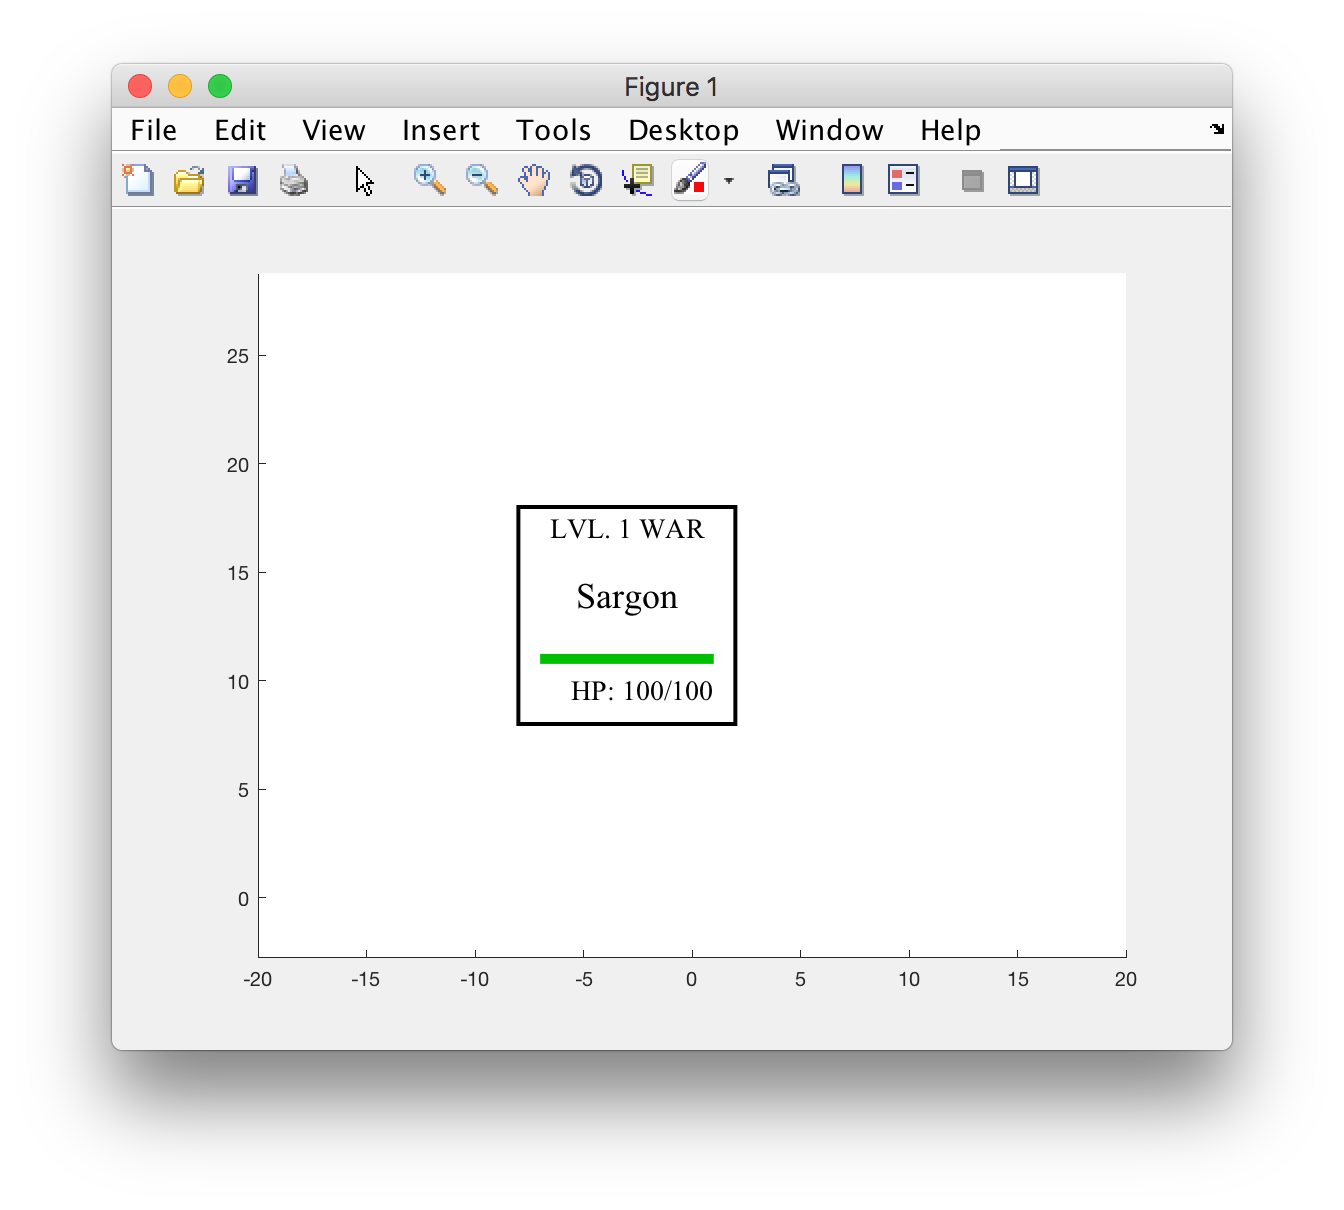
\includegraphics[width=5in]{graphics/AvatarDrawGraphOut.png} 
   \caption{A rudimentary graphical representation for an \texttt{Avatar} object. Here, \texttt{Player1} has the name \texttt{'Sargon'} and is drawn to indicate level 1 status as a warrior with full health (100/100 HP).}
   \label{fig:AvatarDrawing}
\end{figure}
% ^^^------------------------------------------------------------^^^